\documentclass{standalone}
\usepackage{amsfonts,amsmath,amssymb}
\usepackage[slovene]{babel}
\usepackage[utf8]{inputenc}
\usepackage[T1]{fontenc}
  
\usepackage{tikz, verbatim}
\usepackage{pgfplots}
\usetikzlibrary{arrows.meta, calc, positioning, automata}

\newcommand{\subdiv}[3] {
\draw ($ 0.5*#2 + 0.5*#3 $) -- #1;
\draw ($ 0.5*#1 + 0.5*#3 $) -- #2;
\draw ($ 0.5*#1 + 0.5*#2 $) -- #3;
}

\begin{document}

		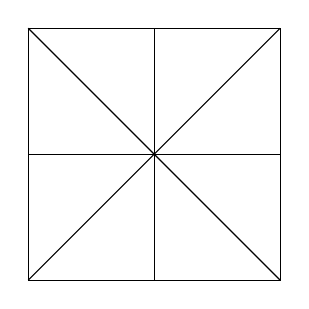
\begin{tikzpicture}[scale=0.4]
		\draw (0, 0) -- (8, 0) -- (8, 8) -- (0, 8) -- (0, 0);
		\draw (4, 0) -- (4, 8);
		\draw (0, 4) -- (8, 4);
		\draw (0, 0) -- (8, 8);
		\draw (0, 8) -- (8, 0);
		\end{tikzpicture}
	
\end{document}